\documentclass{article}
\usepackage{graphicx}
\usepackage{subcaption} % for subfigures


\title{Test Document}
\author{Your Name}
\date{\today}

\begin{document}

\maketitle

\section{Introduction}
This is the AN developed for the CMS analysis for the "Collider-independent asymmetries in the ttbar production".

\section{Looking at the parameters}
There are few parameters that go into the asymmetry equations, like fraction of uubar and ddbar events (Fu and Fd) and detector effect Du and Dd. 
This chapter is dedicated to the study of these parameters and their distributions. 

\subsection{$F_{q}$}
It is mentioned to the fraction of the uubar events in the original paper by author.
Most obvious way to interpret that definition is, fraction of events in which $q\bar{q}$ is the production process for $t\bar{t}$.
i.e. $$F_{q} = \frac{N(q\bar{q}\to t\bar{t})}{N(t\bar{t})}$$ 

At the gen level, we are getting all the ttbar semileptonic events and checking if the parents, i.e. particle 2 and 3 are specific quarks or not.
The distributions of the same for $u$ quark with variation of $|y_{0}|$ for the Run 2 sample are shown in Fig.1\\

\begin{figure}[htbp]
    \centering
    \begin{subfigure}[b]{0.45\textwidth}
        \centering
        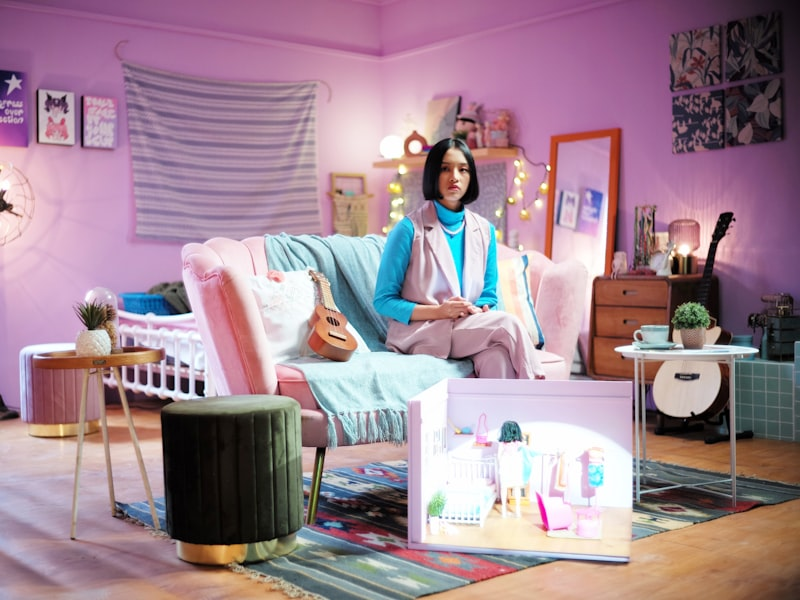
\includegraphics[width=\textwidth]{sample_image.jpg}
        \caption{Caption for Image 1}
        \label{fig:sub1}
    \end{subfigure}
    \begin{subfigure}[b]{0.45\textwidth}
        \centering
        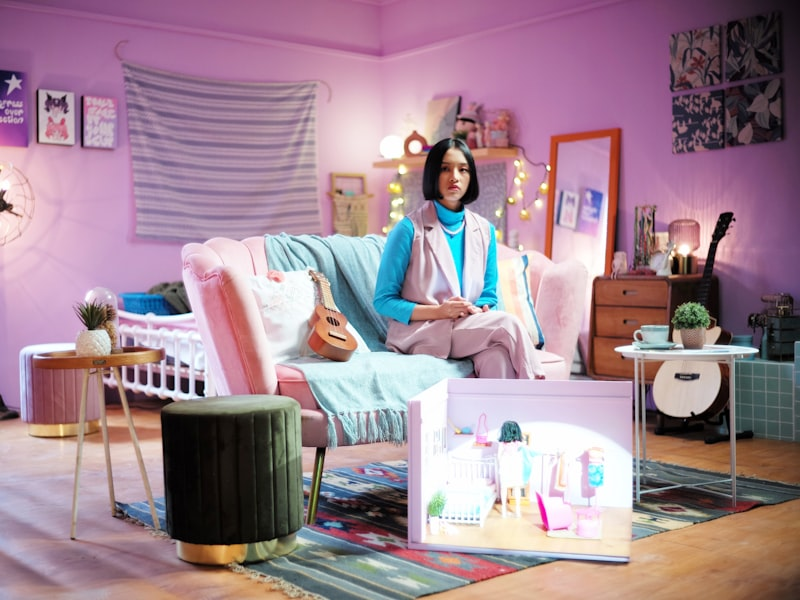
\includegraphics[width=\textwidth]{sample_image.jpg}
        \caption{Caption for Image 2}
        \label{fig:sub2}
    \end{subfigure}

    \begin{subfigure}[b]{0.45\textwidth}
        \centering
        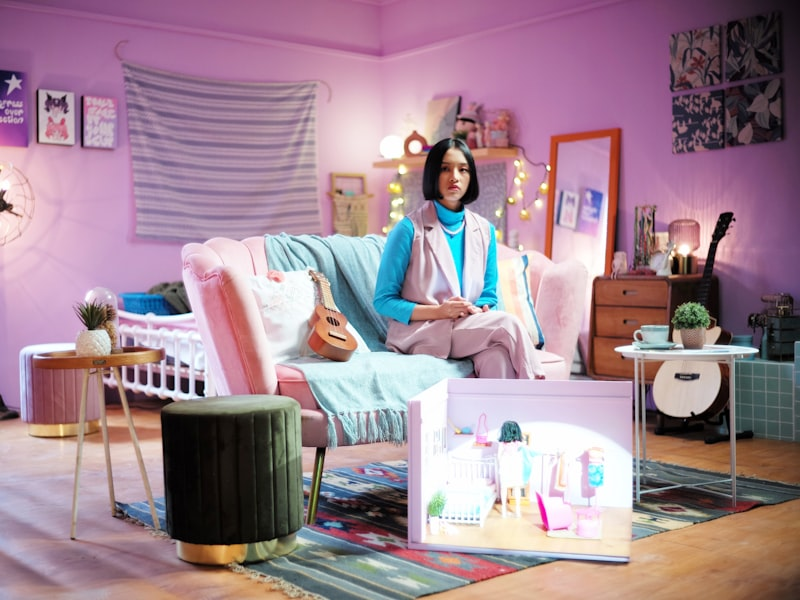
\includegraphics[width=\textwidth]{sample_image.jpg}
        \caption{Caption for Image 3}
        \label{fig:sub3}
    \end{subfigure}
    \begin{subfigure}[b]{0.45\textwidth}
        \centering
        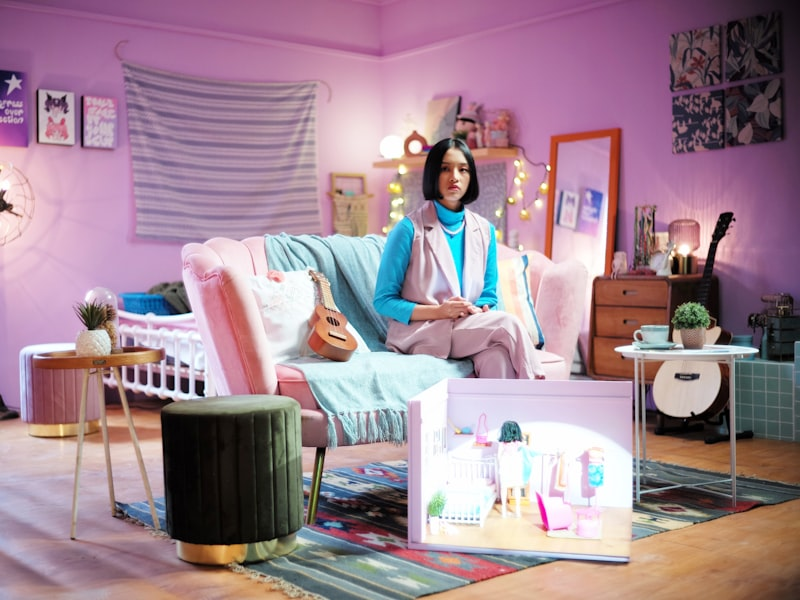
\includegraphics[width=\textwidth]{sample_image.jpg}
        \caption{Caption for Image 4}
        \label{fig:sub4}
    \end{subfigure}
    \caption{Overall Caption for the 2x2 Grid}
    \label{fig:grid}
\end{figure}

\noindent Fig. 2 shows the similar plots for $d$ quark processes.
\\
\begin{figure}[htbp]
    \centering
    \begin{subfigure}[b]{0.45\textwidth}
        \centering
        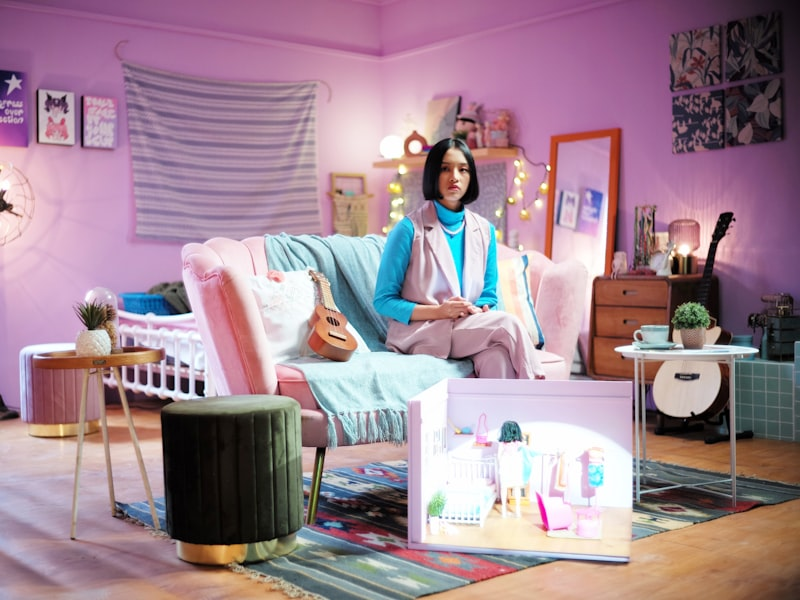
\includegraphics[width=\textwidth]{sample_image.jpg}
        \caption{Caption for Image 1}
        \label{fig:sub1}
    \end{subfigure}
    \begin{subfigure}[b]{0.45\textwidth}
        \centering
        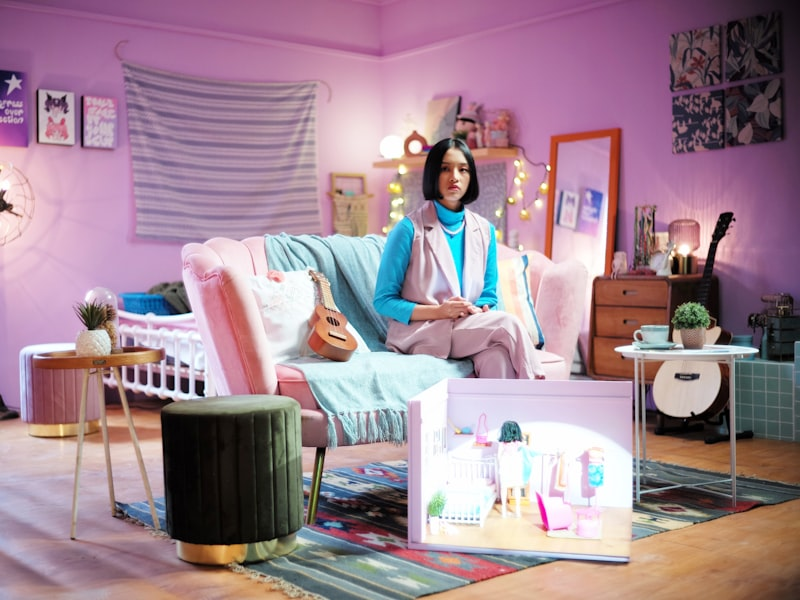
\includegraphics[width=\textwidth]{sample_image.jpg}
        \caption{Caption for Image 2}
        \label{fig:sub2}
    \end{subfigure}

    \begin{subfigure}[b]{0.45\textwidth}
        \centering
        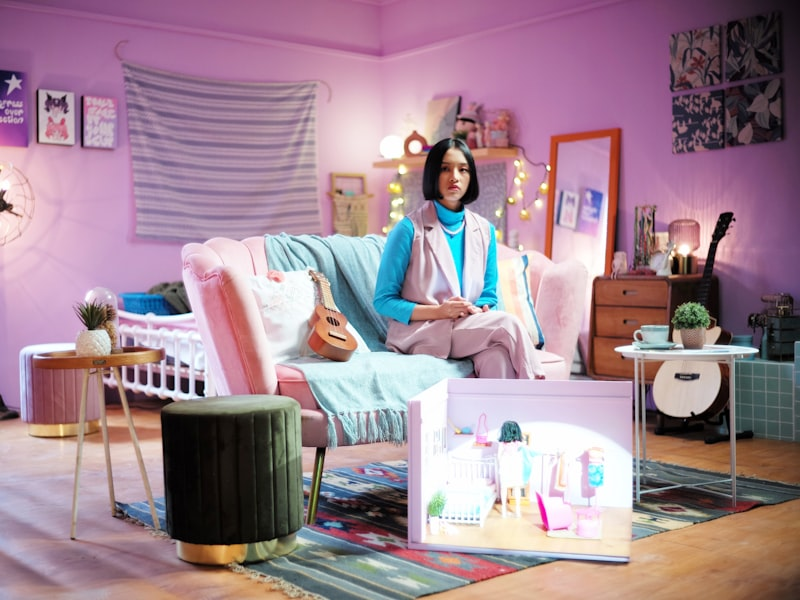
\includegraphics[width=\textwidth]{sample_image.jpg}
        \caption{Caption for Image 3}
        \label{fig:sub3}
    \end{subfigure}
    \begin{subfigure}[b]{0.45\textwidth}
        \centering
        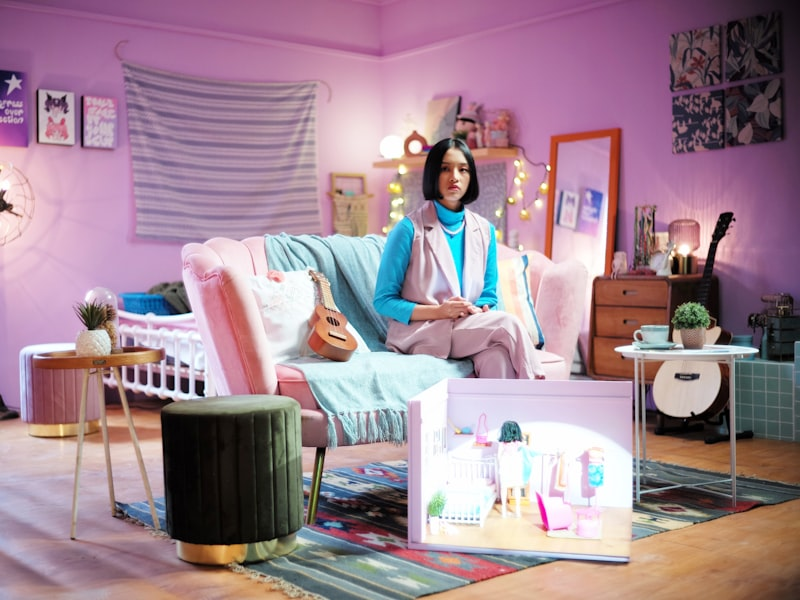
\includegraphics[width=\textwidth]{sample_image.jpg}
        \caption{Caption for Image 4}
        \label{fig:sub4}
    \end{subfigure}
    \caption{Overall Caption for the 2x2 Grid}
    \label{fig:grid}
\end{figure}

\noindent The key feature we want to study is the correlation between these two fractions $F_{u} \ vs \ F_d$. These are shown in Fig.3

For the sake of completion, I also calculated the fractions $F_{q}'$ with only the uubar and ddbar processes in consideration.
i.e. 
$$F_{u}' = \frac{N(u\bar{u})}{N(u\bar{u}) + N(d\bar{d})}$$ 

\noindent Fig. 4 and 5 shows the distribution of these for u and d quarks respectively.

\begin{figure}[htbp]
    \centering
    \begin{subfigure}[b]{0.45\textwidth}
        \centering
        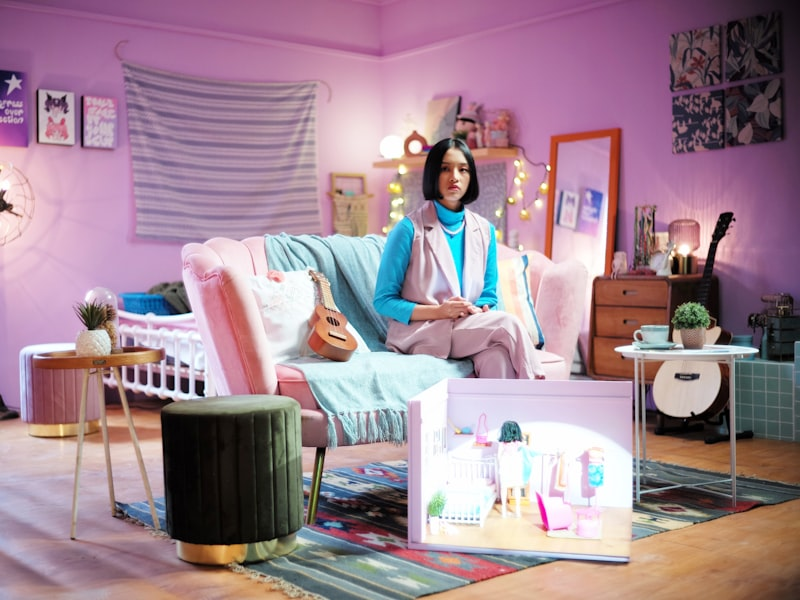
\includegraphics[width=\textwidth]{sample_image.jpg}
        \caption{Caption for Image 1}
        \label{fig:sub1}
    \end{subfigure}
    \begin{subfigure}[b]{0.45\textwidth}
        \centering
        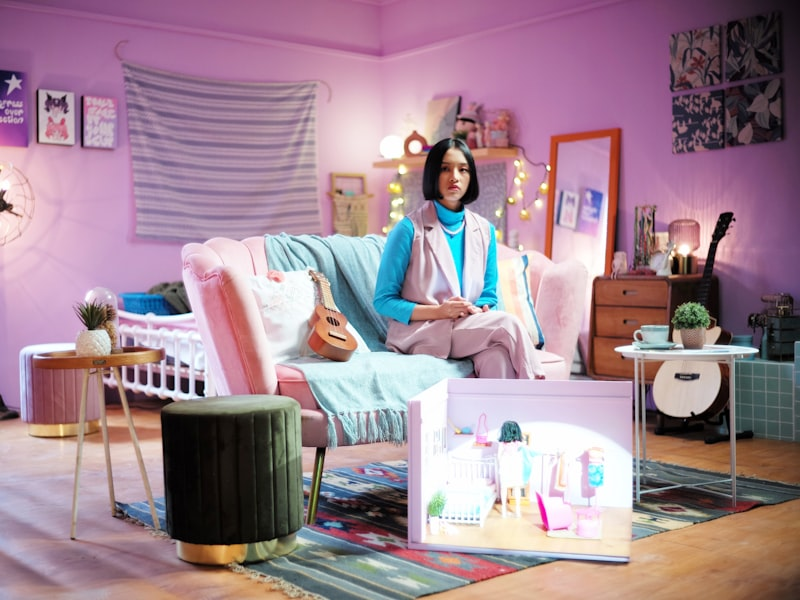
\includegraphics[width=\textwidth]{sample_image.jpg}
        \caption{Caption for Image 2}
        \label{fig:sub2}
    \end{subfigure}

    \begin{subfigure}[b]{0.45\textwidth}
        \centering
        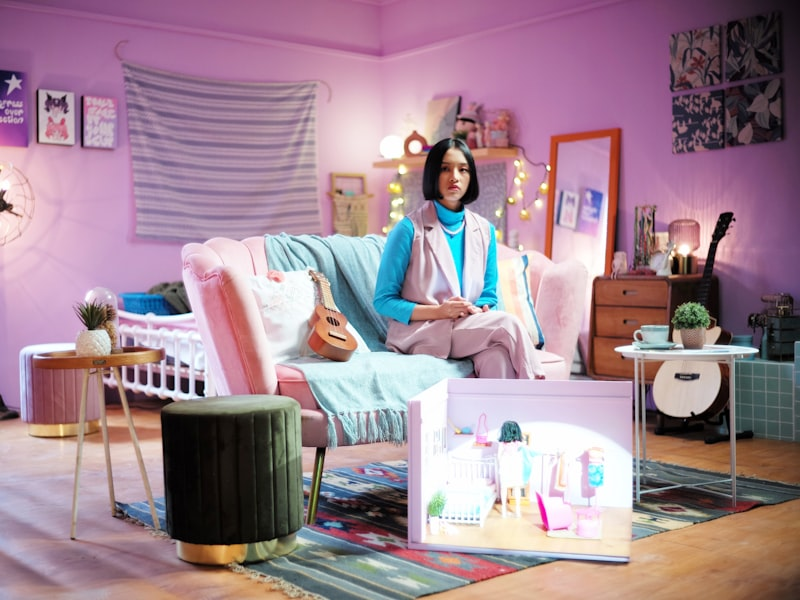
\includegraphics[width=\textwidth]{sample_image.jpg}
        \caption{Caption for Image 3}
        \label{fig:sub3}
    \end{subfigure}
    \begin{subfigure}[b]{0.45\textwidth}
        \centering
        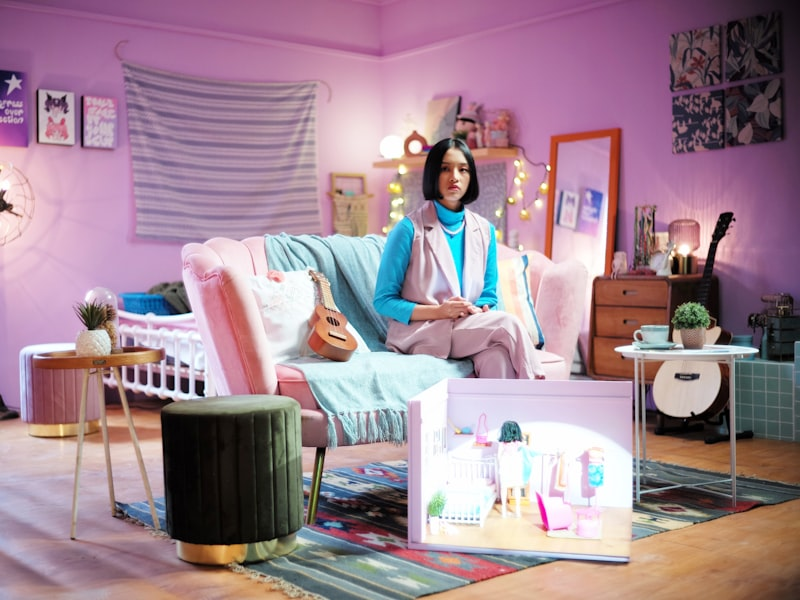
\includegraphics[width=\textwidth]{sample_image.jpg}
        \caption{Caption for Image 4}
        \label{fig:sub4}
    \end{subfigure}
    \caption{Overall Caption for the 2x2 Grid}
    \label{fig:grid}
\end{figure}


\begin{figure}[htbp]
    \centering
    \begin{subfigure}[b]{0.45\textwidth}
        \centering
        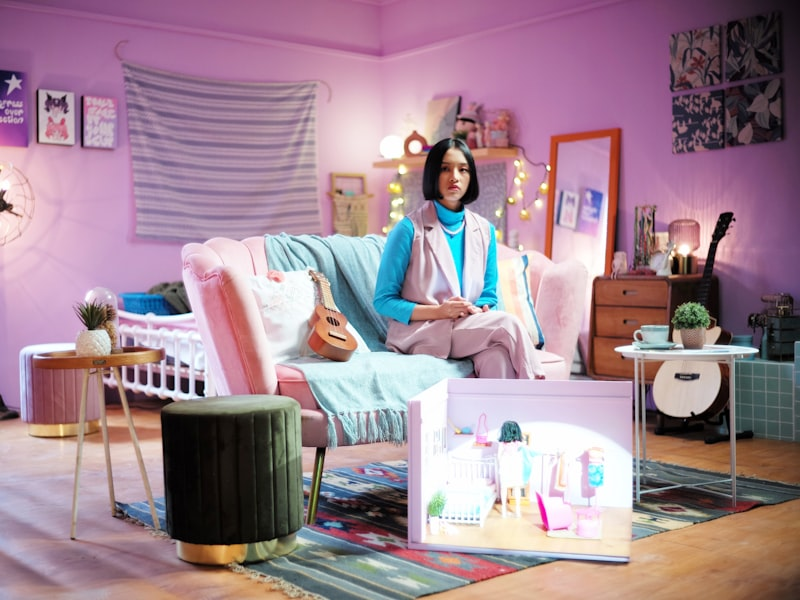
\includegraphics[width=\textwidth]{sample_image.jpg}
        \caption{Caption for Image 1}
        \label{fig:sub1}
    \end{subfigure}
    \begin{subfigure}[b]{0.45\textwidth}
        \centering
        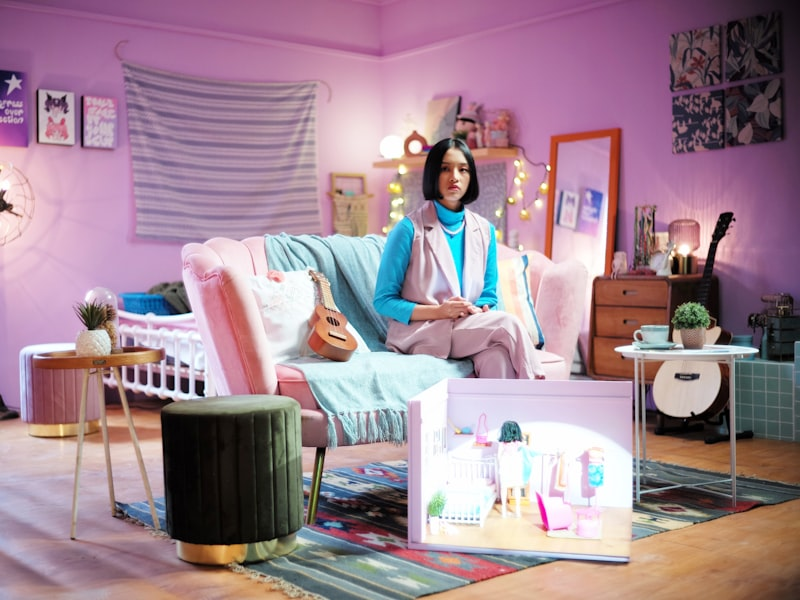
\includegraphics[width=\textwidth]{sample_image.jpg}
        \caption{Caption for Image 2}
        \label{fig:sub2}
    \end{subfigure}

    \begin{subfigure}[b]{0.45\textwidth}
        \centering
        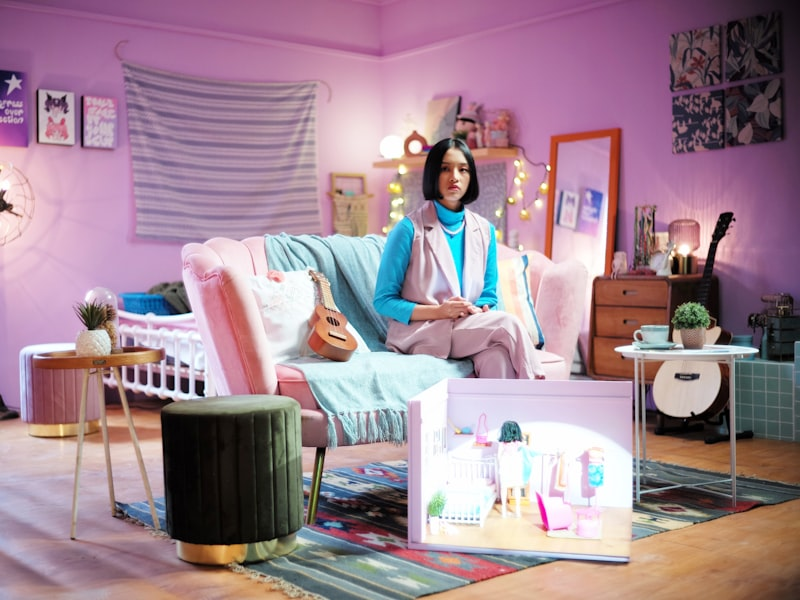
\includegraphics[width=\textwidth]{sample_image.jpg}
        \caption{Caption for Image 3}
        \label{fig:sub3}
    \end{subfigure}
    \begin{subfigure}[b]{0.45\textwidth}
        \centering
        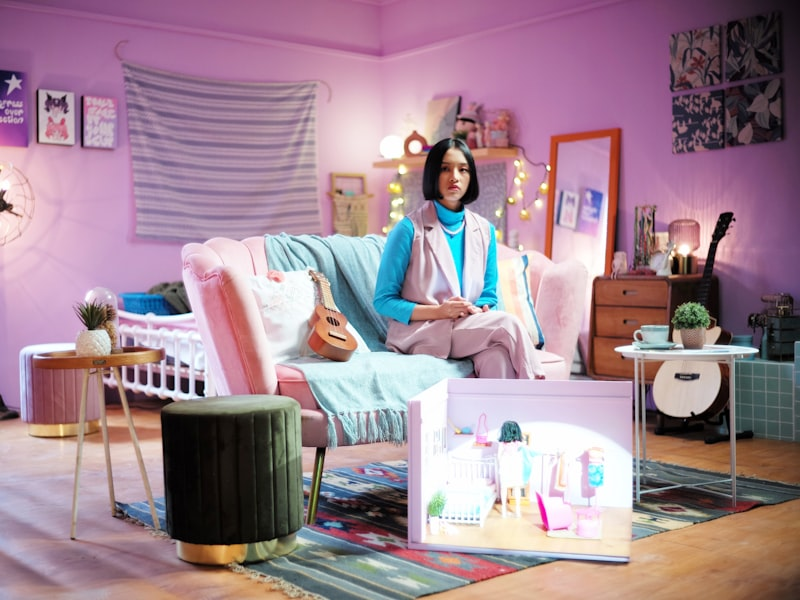
\includegraphics[width=\textwidth]{sample_image.jpg}
        \caption{Caption for Image 4}
        \label{fig:sub4}
    \end{subfigure}
    \caption{Overall Caption for the 2x2 Grid}
    \label{fig:grid}
\end{figure}

\subsection*{$D_q$}
The other parameter that we are using in the model is $D_q$, which is supposed to quantify the detector effect.
In the theory paper it is defined as the relative difference between the events with higher quark momentum than antiquark momentum.
we interpreted it as 
$$D = \frac{N(x_q > x_{\bar{q}}) - N(x_q > x_{\bar{q}})}{N(x_q > x_{\bar{q}}) + N(x_q > x_{\bar{q}})}$$

The obtained distribution of $D_u$ and $D_d$ is shown in Fig. 6 and 7 with variation of $|y_0|$. Fig. 8 shows the correlation between $D_u$ and $D_d$

\begin{figure}[htbp]
    \centering
    \begin{subfigure}[b]{0.45\textwidth}
        \centering
        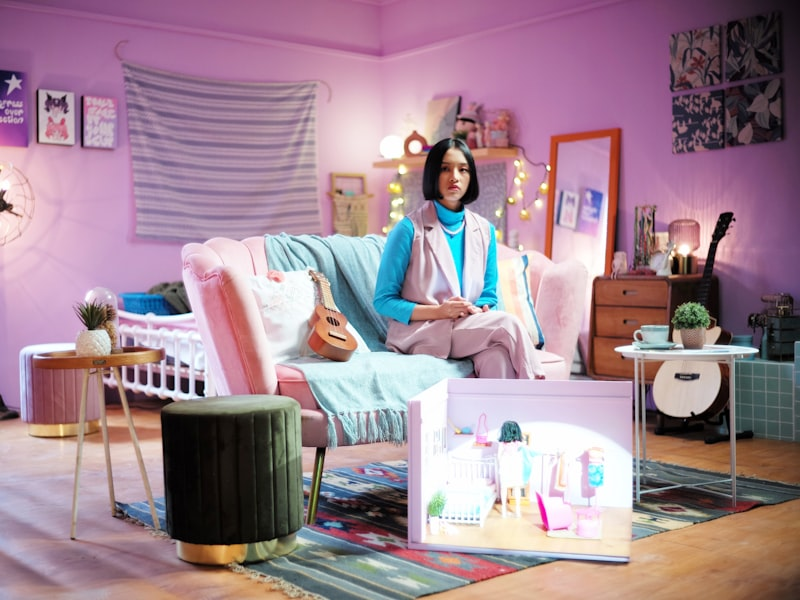
\includegraphics[width=\textwidth]{sample_image.jpg}
        \caption{Caption for Image 1}
        \label{fig:sub1}
    \end{subfigure}
    \begin{subfigure}[b]{0.45\textwidth}
        \centering
        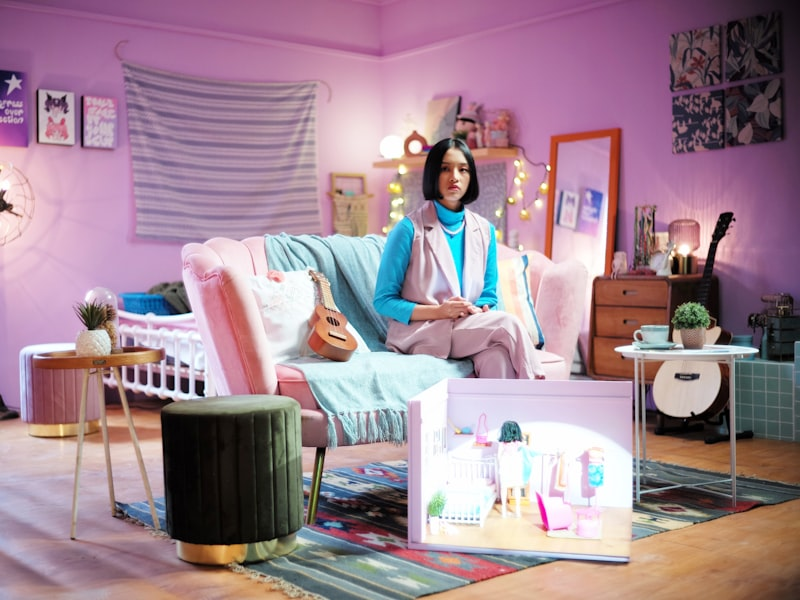
\includegraphics[width=\textwidth]{sample_image.jpg}
        \caption{Caption for Image 2}
        \label{fig:sub2}
    \end{subfigure}

    \begin{subfigure}[b]{0.45\textwidth}
        \centering
        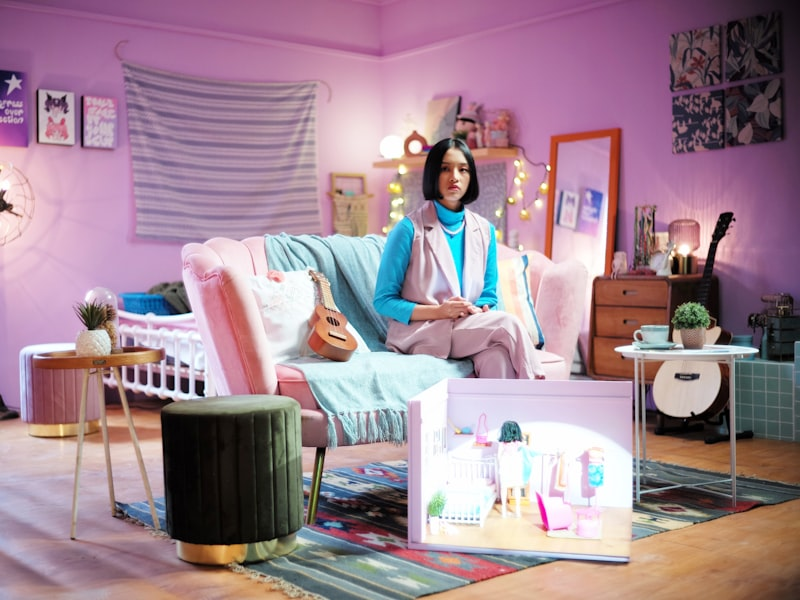
\includegraphics[width=\textwidth]{sample_image.jpg}
        \caption{Caption for Image 3}
        \label{fig:sub3}
    \end{subfigure}
    \begin{subfigure}[b]{0.45\textwidth}
        \centering
        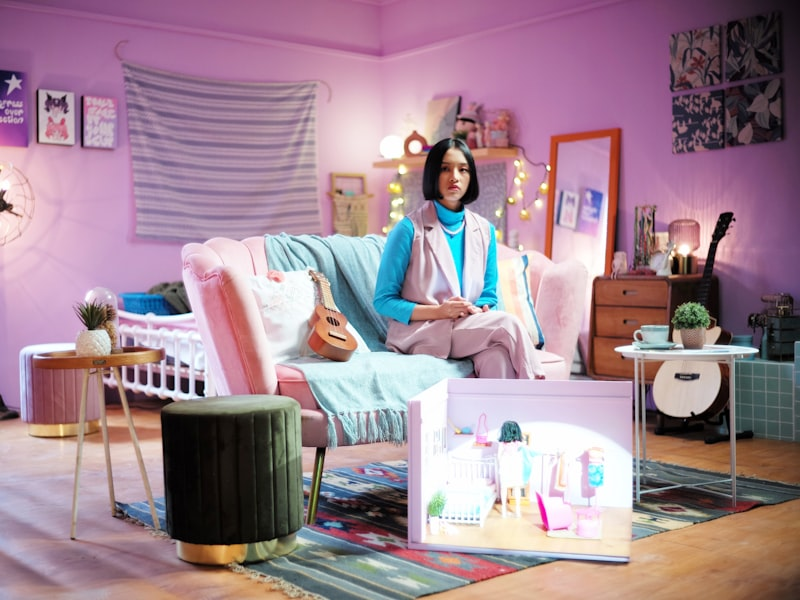
\includegraphics[width=\textwidth]{sample_image.jpg}
        \caption{Caption for Image 4}
        \label{fig:sub4}
    \end{subfigure}
    \caption{Overall Caption for the 2x2 Grid}
    \label{fig:grid}
\end{figure}

\begin{figure}[htbp]
    \centering
    \begin{subfigure}[b]{0.45\textwidth}
        \centering
        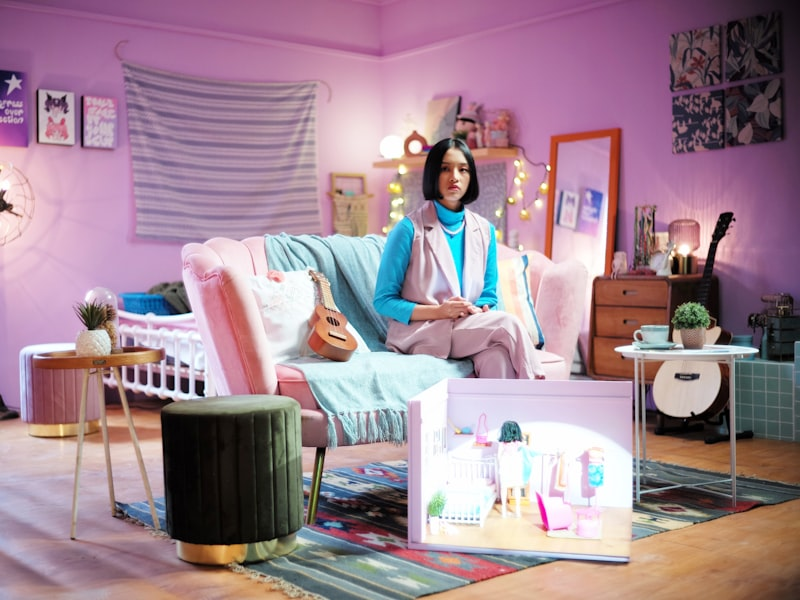
\includegraphics[width=\textwidth]{sample_image.jpg}
        \caption{Caption for Image 1}
        \label{fig:sub1}
    \end{subfigure}
    \begin{subfigure}[b]{0.45\textwidth}
        \centering
        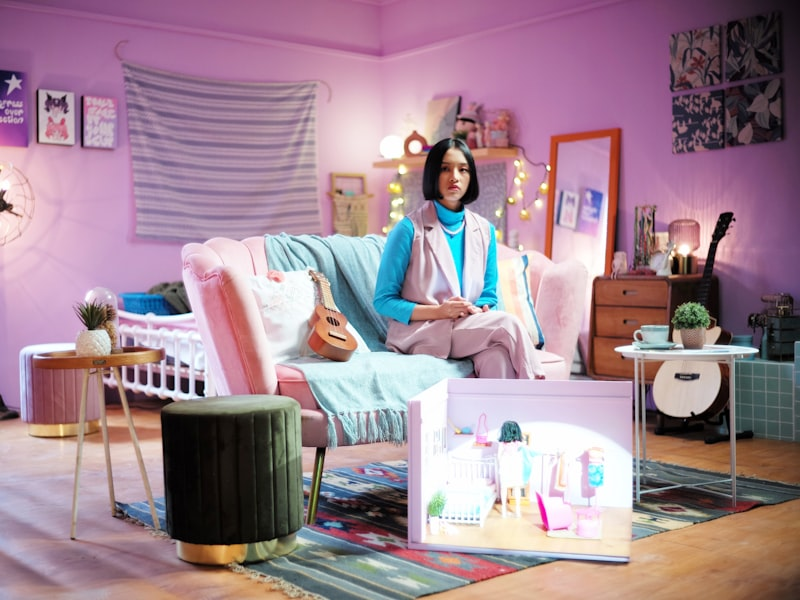
\includegraphics[width=\textwidth]{sample_image.jpg}
        \caption{Caption for Image 2}
        \label{fig:sub2}
    \end{subfigure}

    \begin{subfigure}[b]{0.45\textwidth}
        \centering
        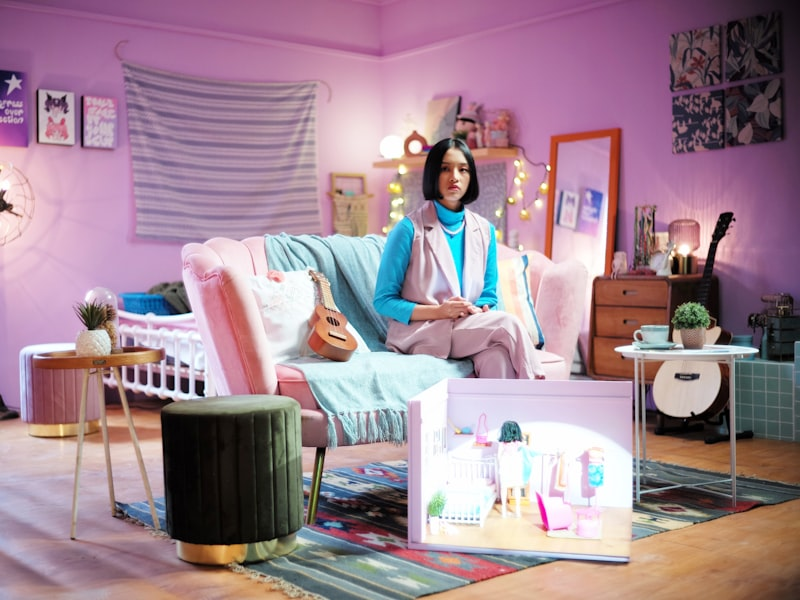
\includegraphics[width=\textwidth]{sample_image.jpg}
        \caption{Caption for Image 3}
        \label{fig:sub3}
    \end{subfigure}
    \begin{subfigure}[b]{0.45\textwidth}
        \centering
        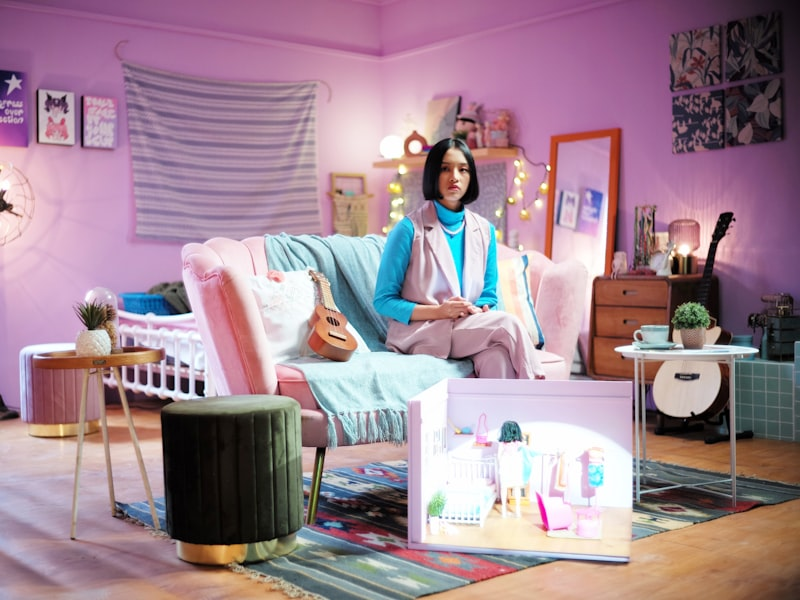
\includegraphics[width=\textwidth]{sample_image.jpg}
        \caption{Caption for Image 4}
        \label{fig:sub4}
    \end{subfigure}
    \caption{Overall Caption for the 2x2 Grid}
    \label{fig:grid}
\end{figure}
    
\begin{figure}
    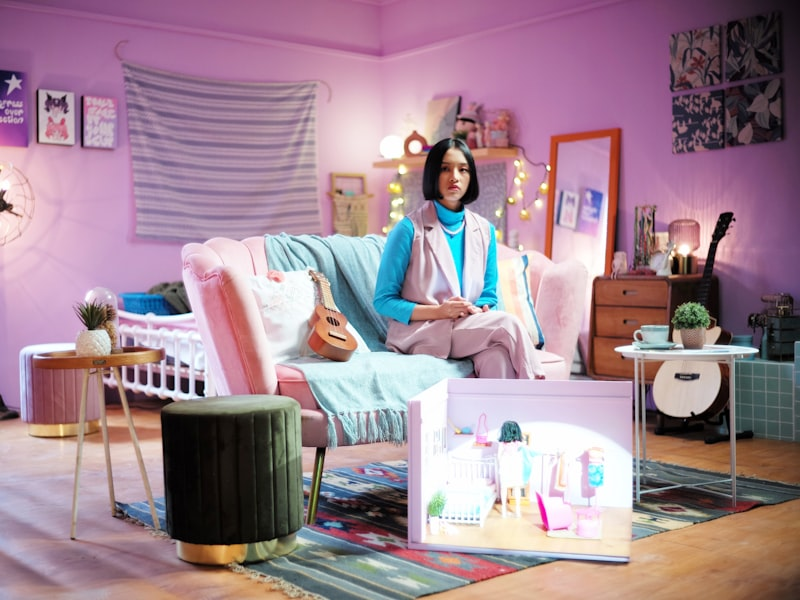
\includegraphics[width=\textwidth]{sample_image.jpg}
\end{figure}

\end{document}

